\documentclass{article}
\usepackage[utf8]{inputenc}
\usepackage{graphicx}
\graphicspath{.}
\usepackage{amsmath}
\usepackage{hyperref}
\usepackage{amssymb}
\usepackage{xcolor}
\title{ECE310 Final Review - Cramming Carnival Solutions}
\author{Author: Members of HKN}
\date{}
\newcommand{\dd}[1]{\mathrm{d}#1}

\usepackage[makeroom]{cancel}
\usepackage[letterpaper, portrait, margin=1in]{geometry}

\pagenumbering{arabic}

\begin{document}

\maketitle

\begin{figure}[h]
\begin{center}
    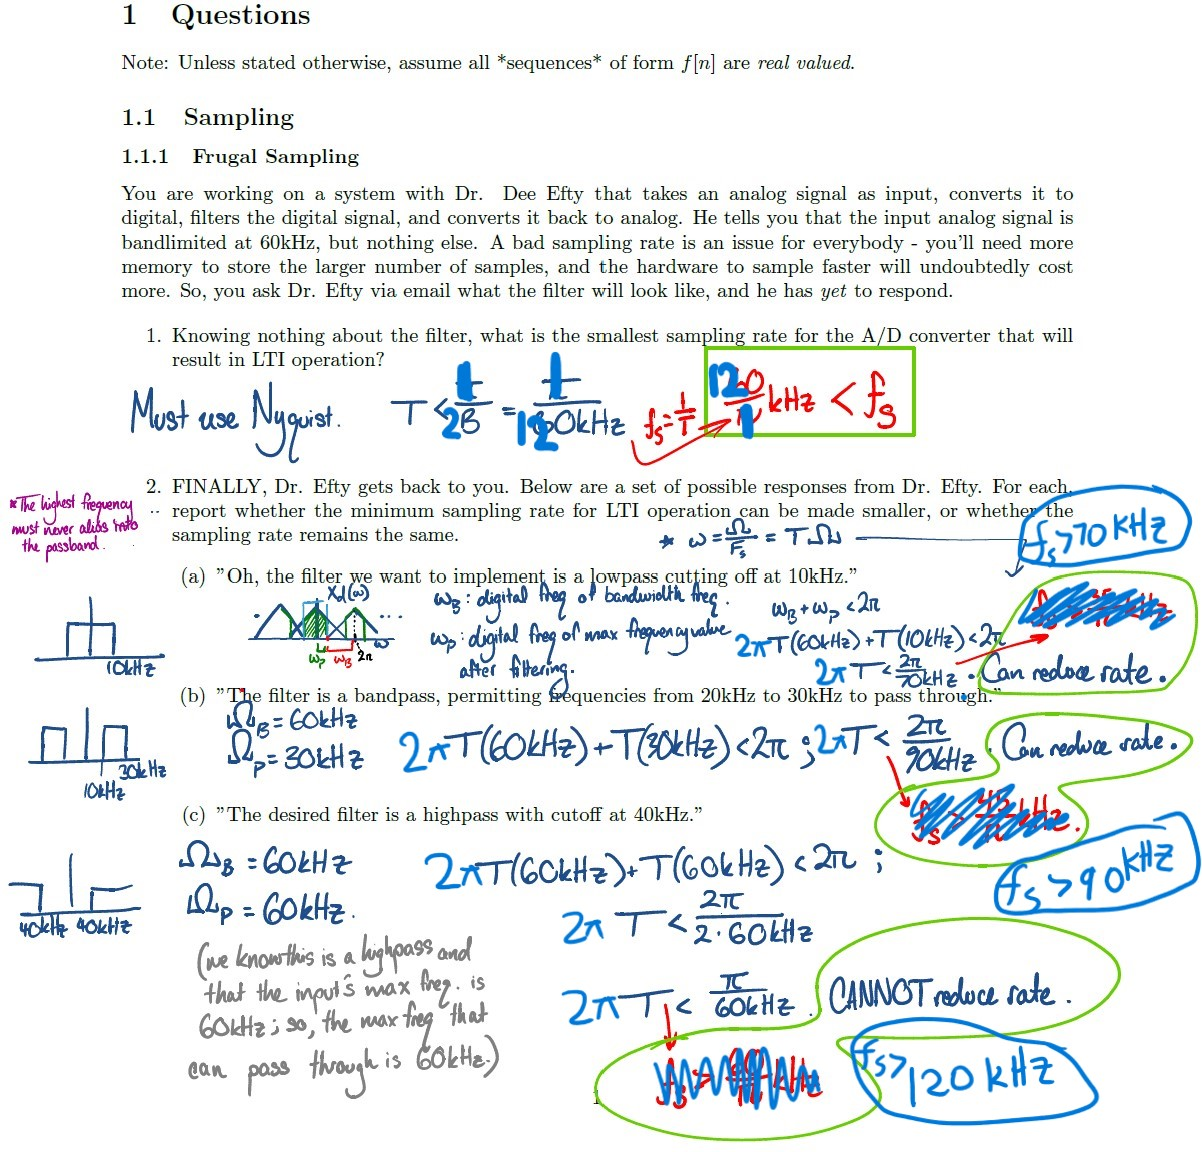
\includegraphics[width=0.96 \textwidth]{figures/Solutions pg 1.jpg}
    \label{fig:old_solutions_1}
\end{center}
\end{figure}

\newpage

\begin{figure}[h!]
\begin{center}
    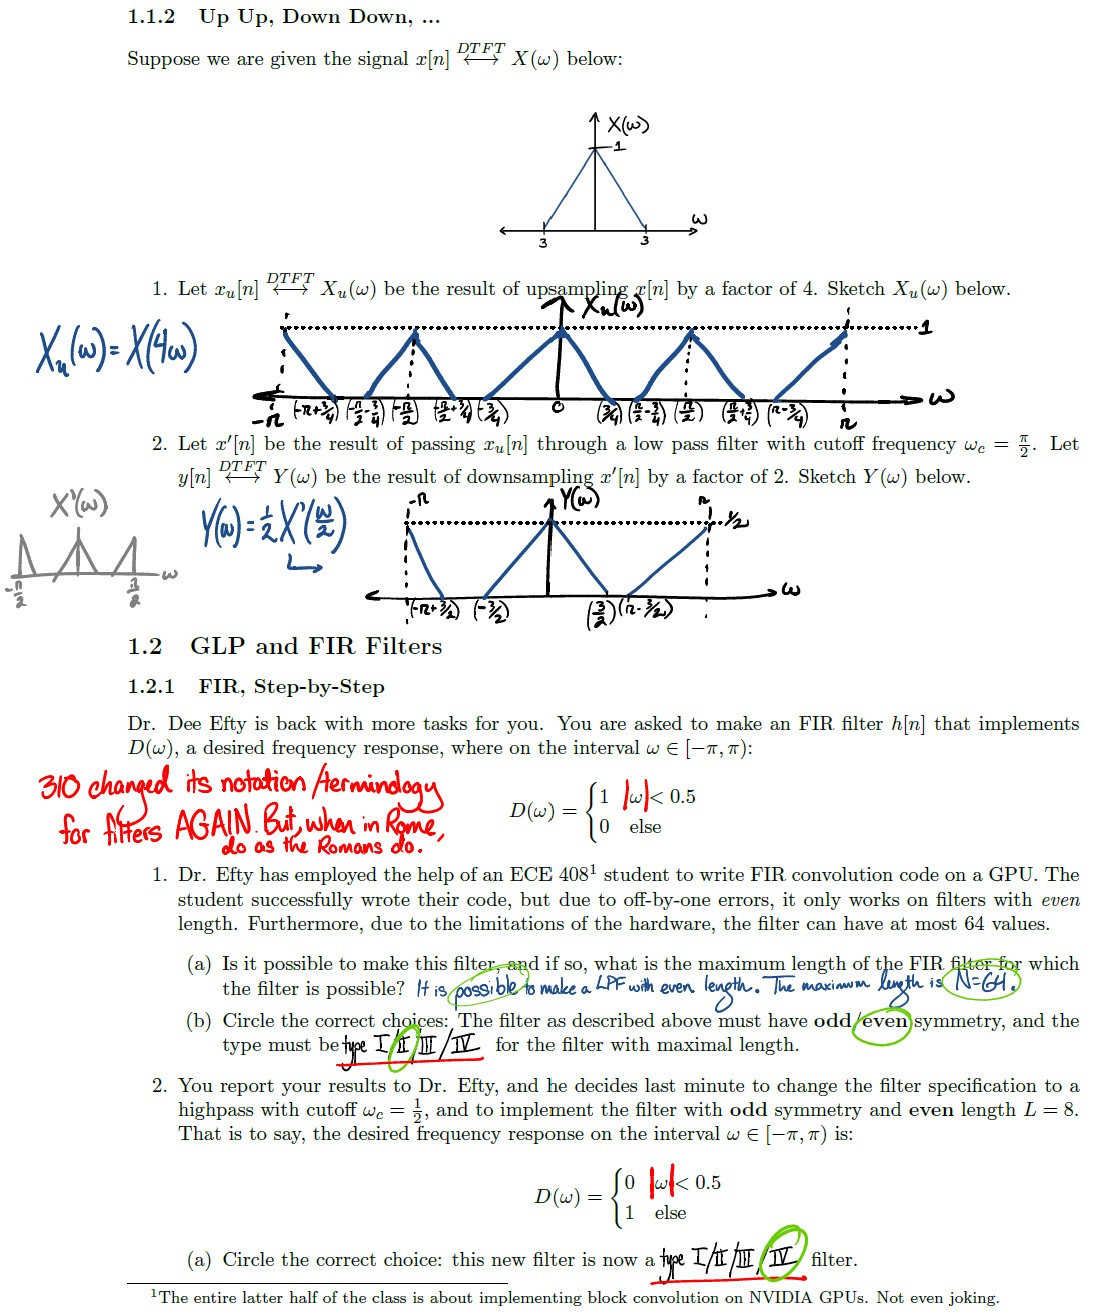
\includegraphics[width= \textwidth]{figures/Solutions pg 2.jpg}
    \label{fig:old_solutions_2}
\end{center}
\end{figure}

\newpage

\begin{figure}[h!]
\begin{center}
    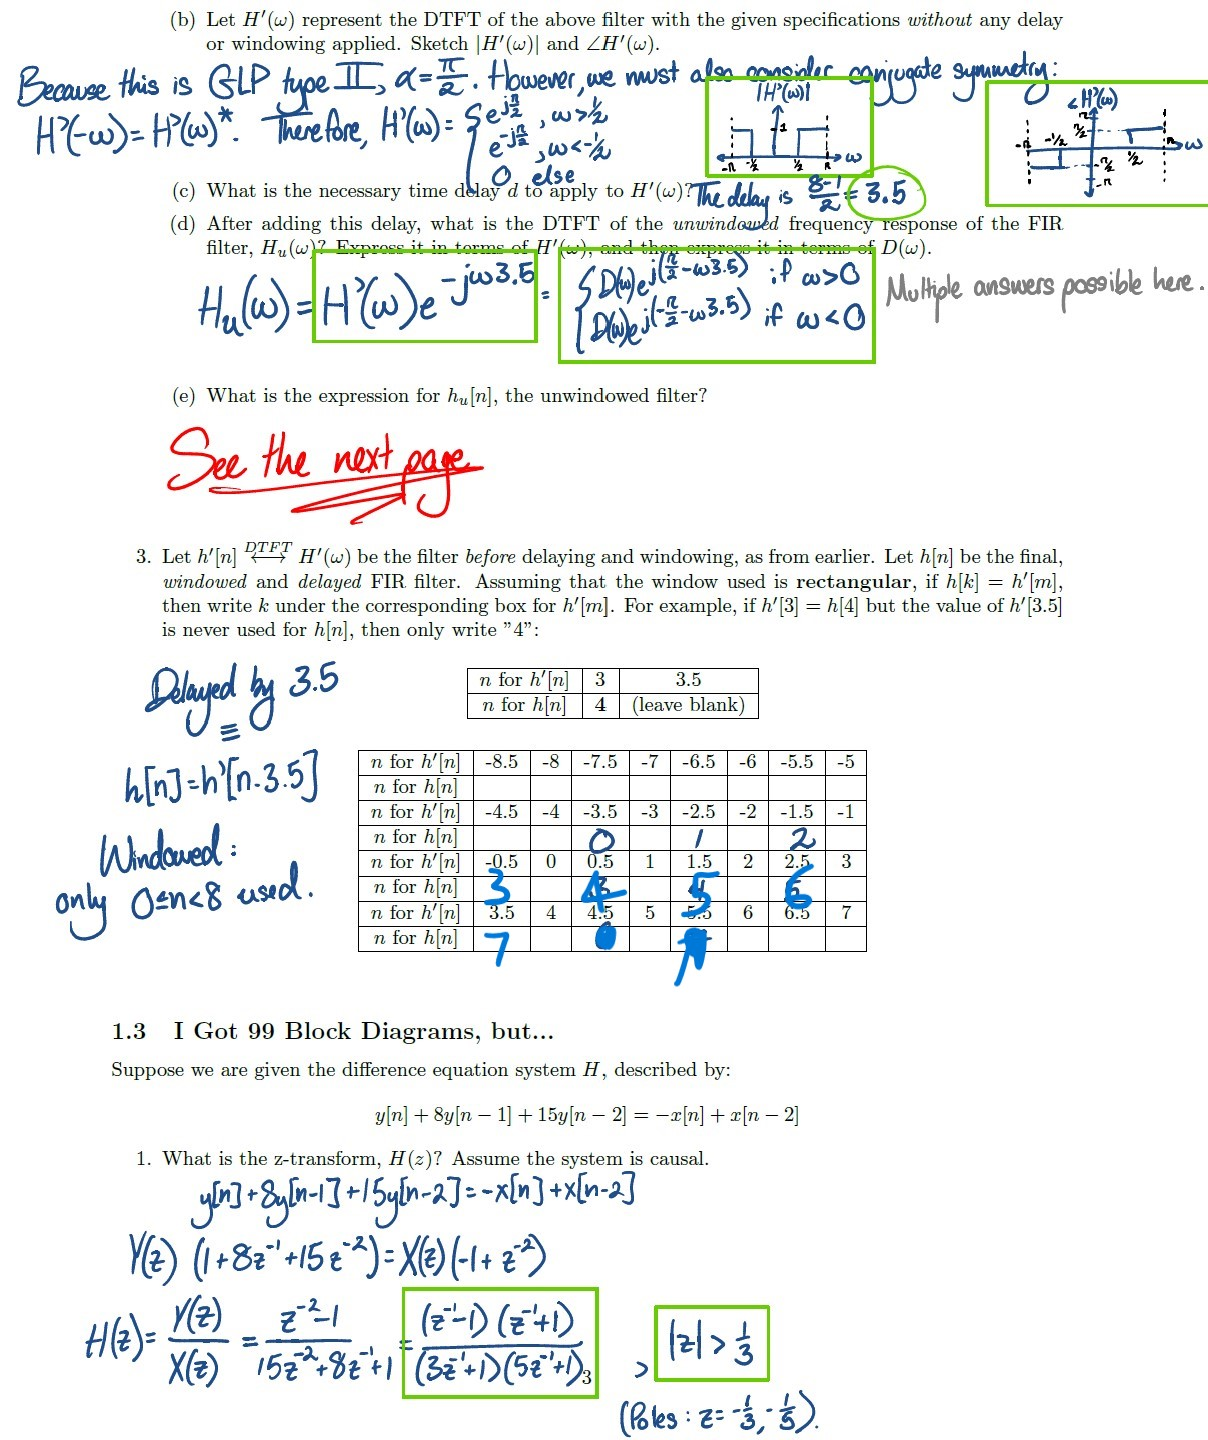
\includegraphics[width= \textwidth]{figures/Solutions pg 3.jpg}
    \label{fig:old_solutions_3}
\end{center}
\end{figure}

\newpage

\begin{figure}[h!]
\begin{center}
    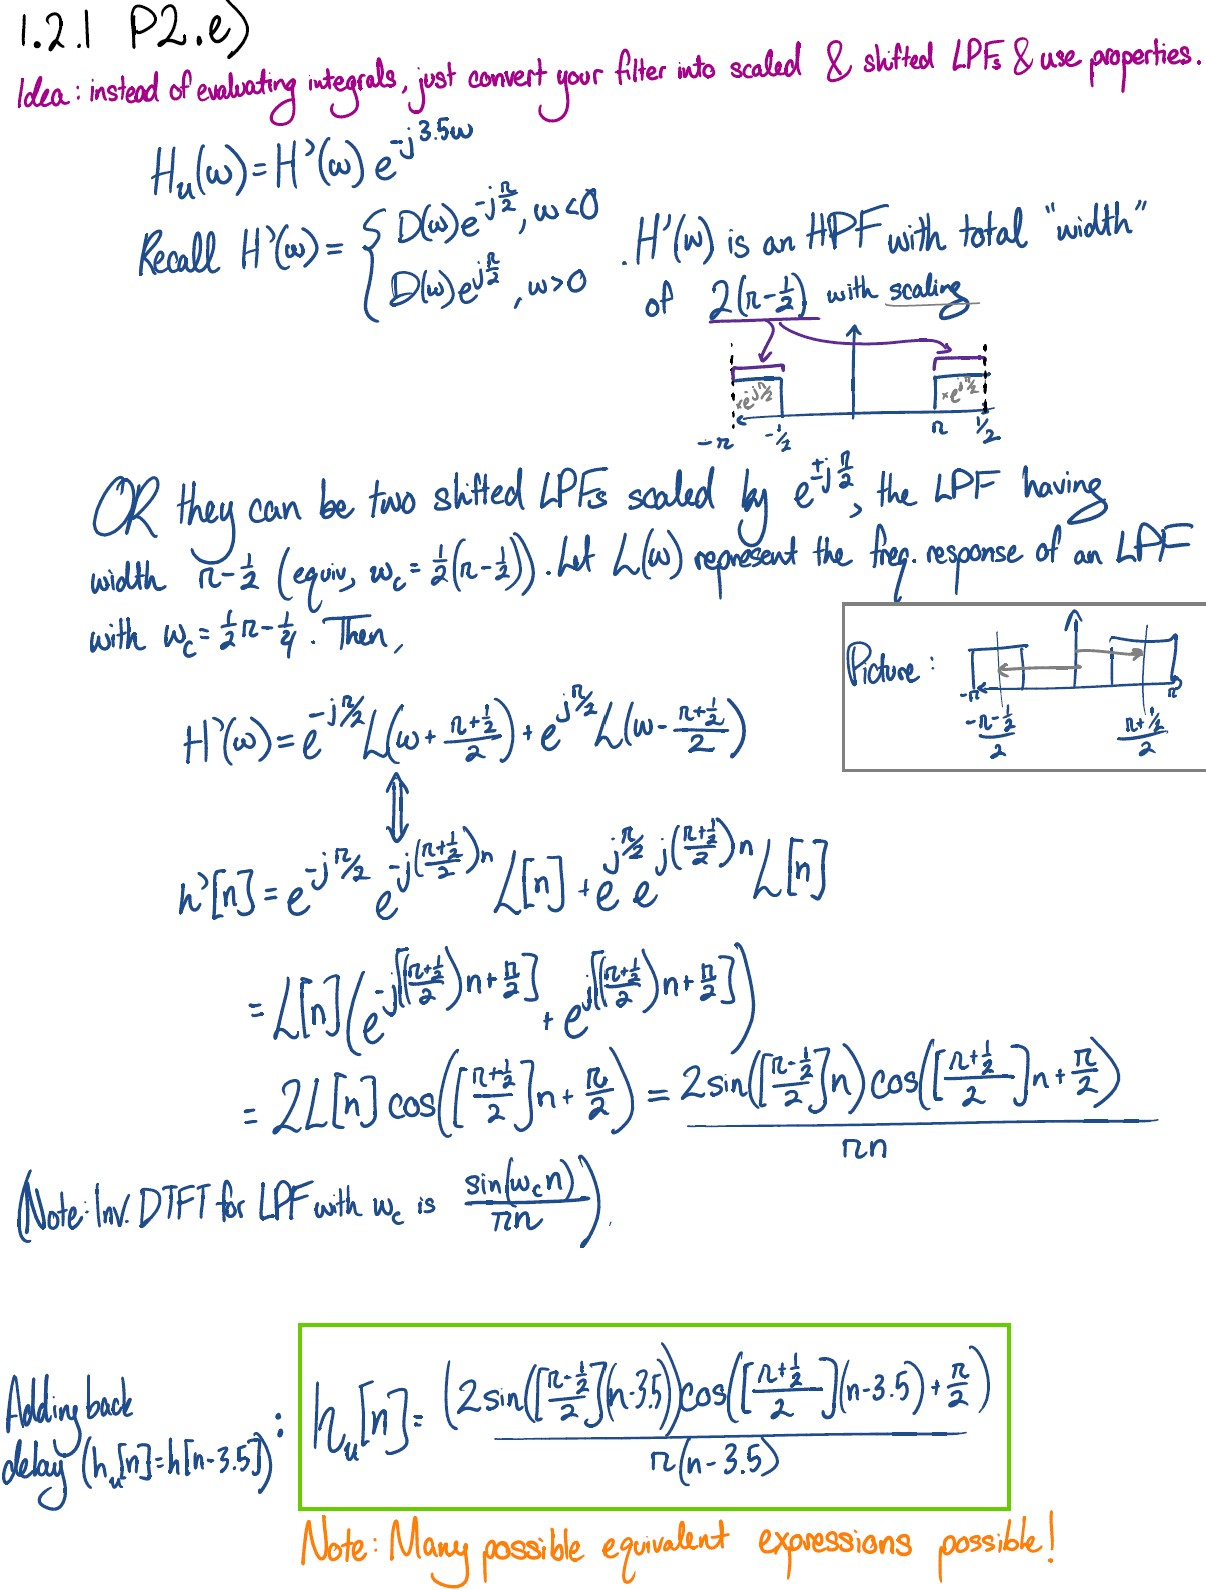
\includegraphics[width=0.99 \textwidth]{figures/Solutions pg 4.jpg}
    \label{fig:old_solutions_4}
\end{center}
\end{figure}

\newpage

\begin{figure}[h!]
\begin{center}
    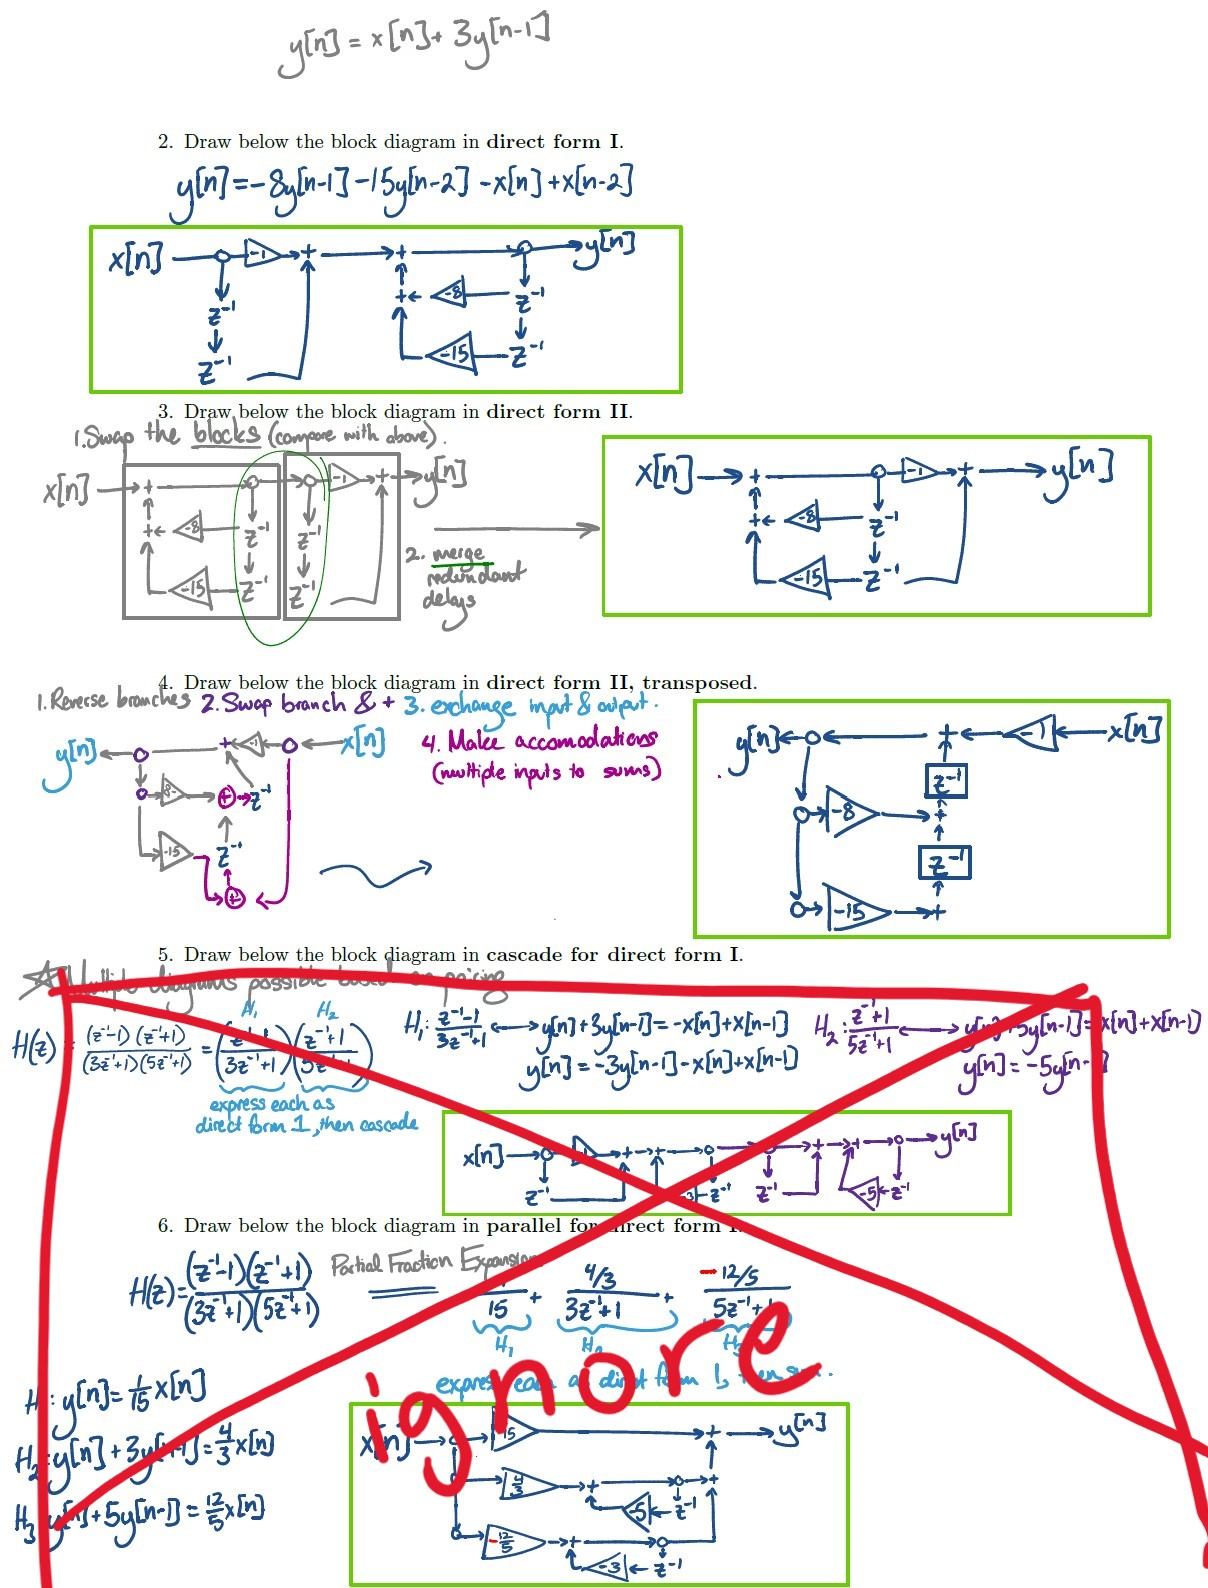
\includegraphics[width=0.99 \textwidth]{figures/Solutions pg 5 Real.jpg}
    \label{fig:old_solutions_5}
\end{center}
\end{figure}

\newpage

\begin{figure}[h]
\begin{center}
    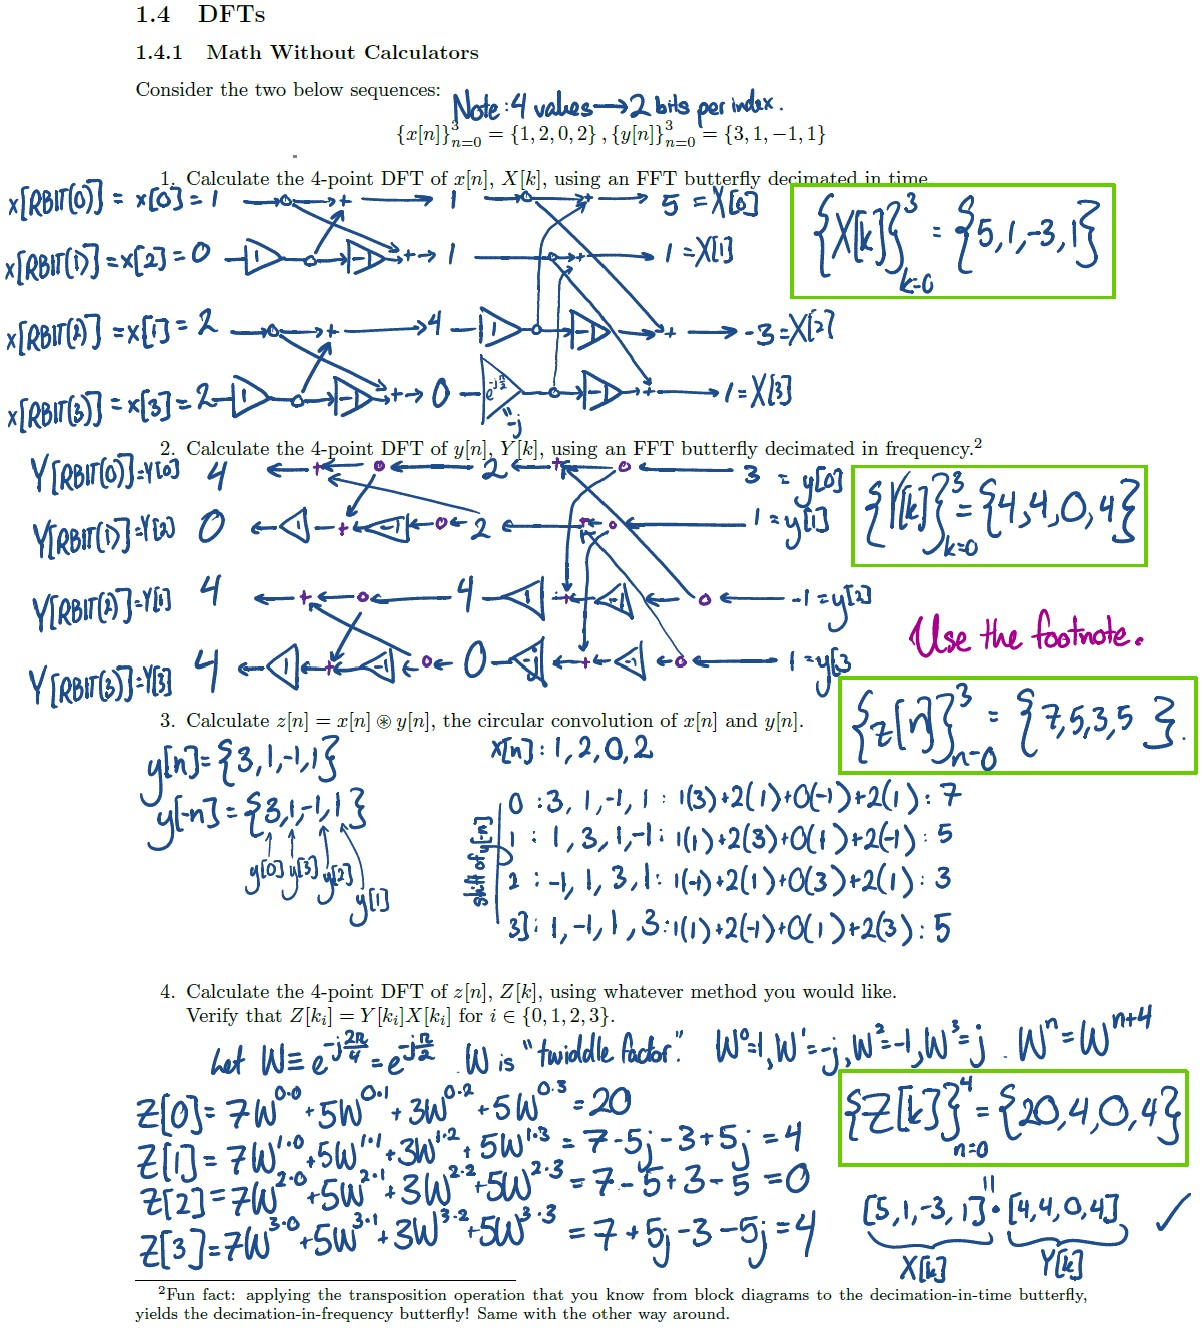
\includegraphics[width=0.95 \textwidth]{figures/Solutions pg 6.jpg}
    \label{fig:old_solutions_6}
\end{center}
\end{figure}

\newpage

\begin{figure}[h]
\begin{center}
    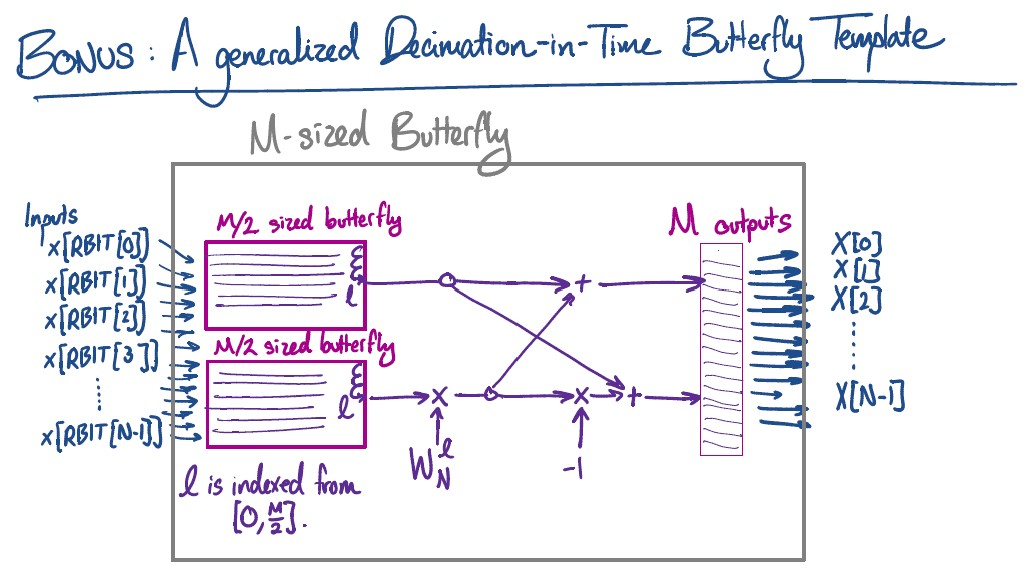
\includegraphics[width= \textwidth]{figures/Solutions pg 7.jpg}
    \label{fig:old_solutions_7}
\end{center}
\end{figure}

\newpage

\section{Famous FFTs}

After a wonderful dinner with Dr. Efty, where the two of you discussed important applications of the FFT, you retire back to your room with an important napkin. On the napkin is a beautiful diagram that Dr. Efty had given to you as a proof for a most illuminating theorem. Unfortunately, during the scramble to figure out who was going to pay, some Sprite got on the napkin. Below is remainder of the diagram.

You recall that the diagram was once part of a 64-bit decimation in time radix-2 FFT. You must find the values of the red letters and greek letters so that you can publish another paper.

\begin{figure}[h!]
\begin{center}
    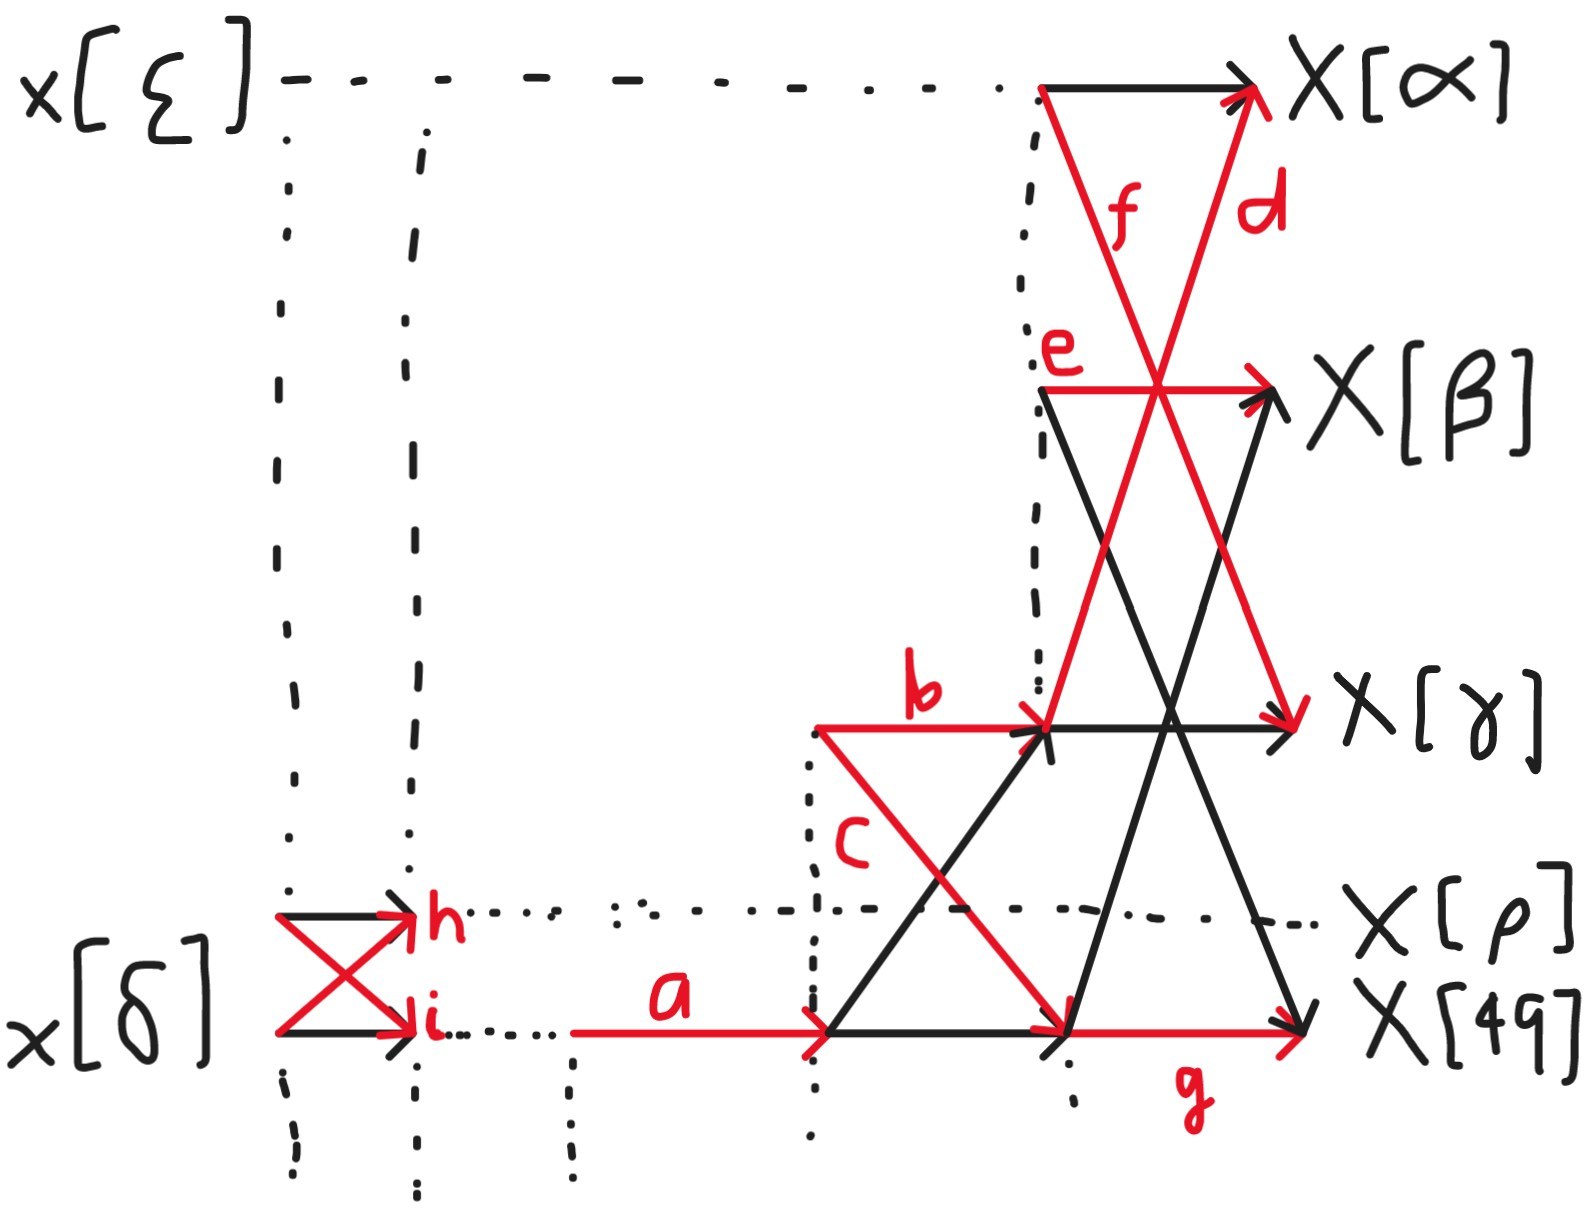
\includegraphics[width=0.8 \textwidth]{figures/FFT Diagram.jpg}
    \caption{The Remains of the Napkin}
    \label{fig:FFT_diagram}
\end{center}
\end{figure}

\subsection{Solution:}

\begin{figure}[h!]
\begin{center}
    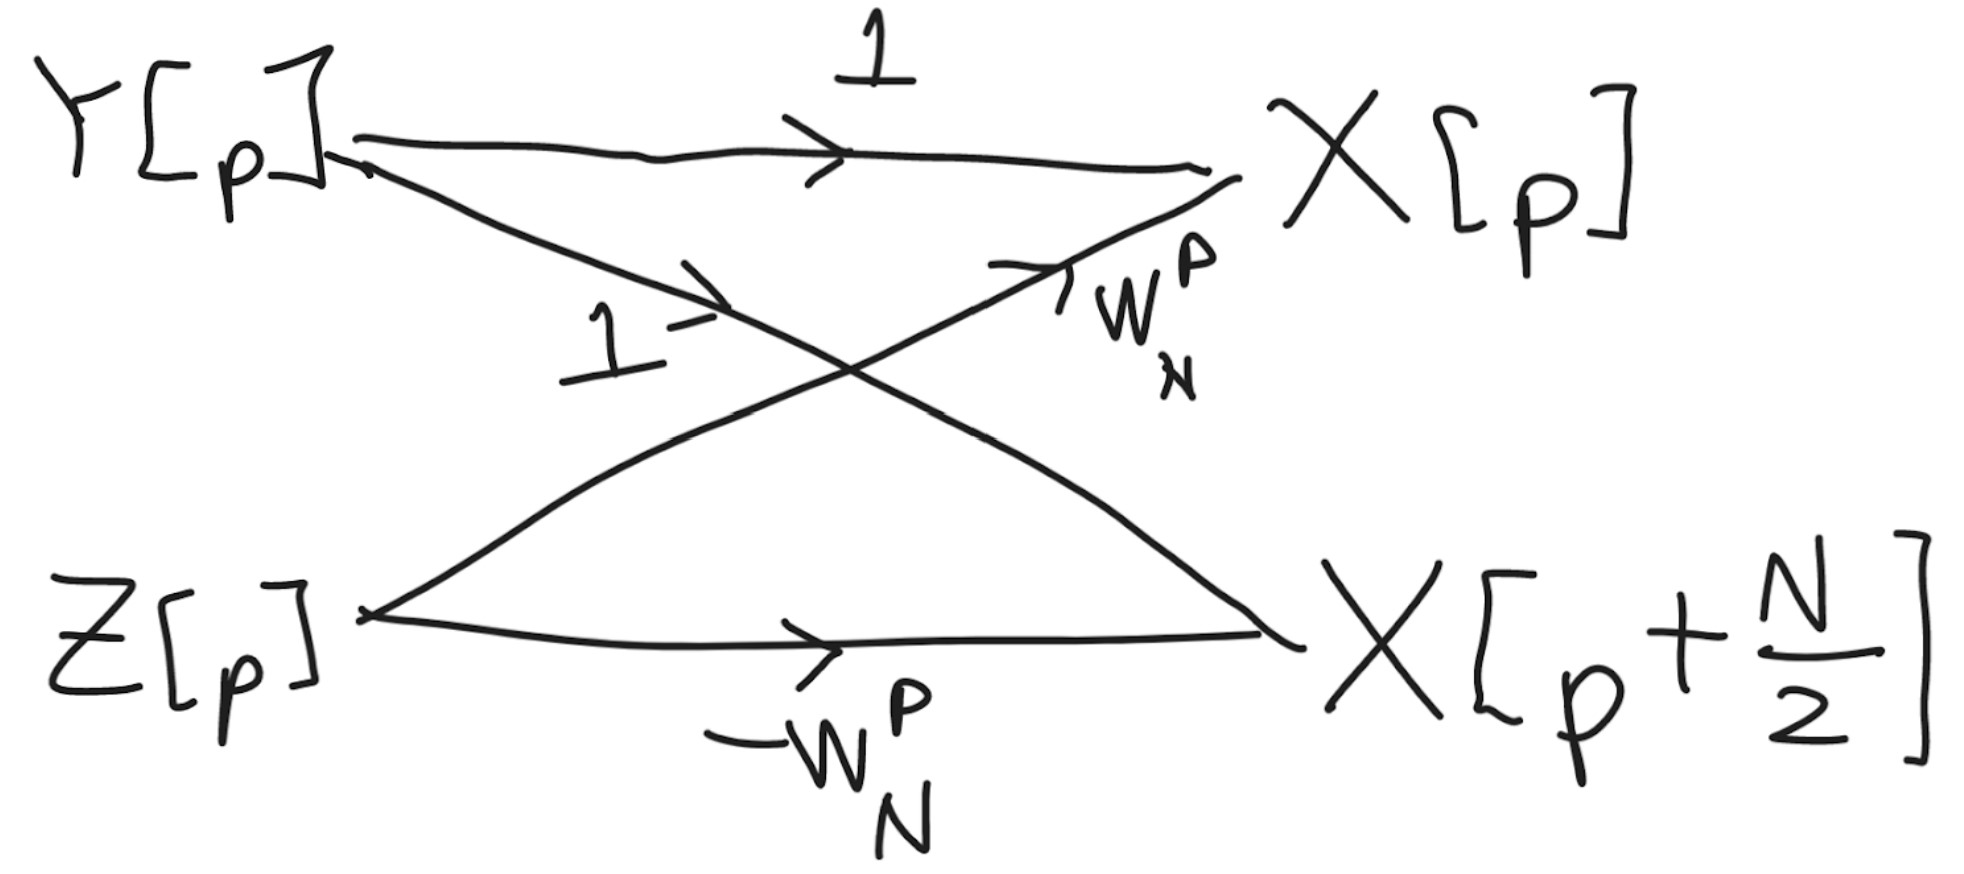
\includegraphics[width=0.5 \textwidth]{figures/FFT Butterfly.jpg}
    \caption{FFT Decimation-in-Time Butterfly}
    \label{fig:FFT Butterfly}
\end{center}
\end{figure}

Figure \ref{fig:FFT Butterfly} shows the FFT butterfly. Let us now solve the problem.

\begin{enumerate}
    \item We know that $X[\beta]$ and $X[49]$ are connected by the final FFT. This means that $\beta + \frac{64}{2} = 49$. Solving, we get $\boxed{\beta = 17}$.
    
    \item We know that $X[\gamma]$ and $X[49]$ are connected by the second to last FFT. This means that $\gamma + \frac{64}{4} = 49$. Solving, we get $\boxed{\gamma = 33}$.
    
    \item We know that $X[\gamma]$ and $X[\alpha]$ are connected by the final FFT. This means that $\alpha + \frac{64}{2} = \gamma$. Using the previous part's solution, we get $\boxed{\alpha = 1}$.
    
    \item FFT input indices are the bit reversal of their output index. Thus, $\epsilon$ is the bit-reversal of $\alpha$ and $\delta$ is the bit reversal of $49$. Solving, we get $\boxed{\epsilon = 32, \delta = 35}$.
    
    \item We know that $x[\delta]$ and the element below it are connected by the first FFT. This means that $X[49]$ and $X[\rho]$ are also right next to each other. Since $49$ is odd, we then know that $\rho + 1 = 49$, so $\boxed{\rho = 48}$.
    
    \item Let's do the easier letters first, i.e. the letters that are on the top of the butterfly or pointing upwards. Matching the arrows with the corresponding arrows in the FFT butterfly diagram, we get $\boxed{b = 1, e = 1, f = 1, c = 1, i = 1}$.
    
    \item We know that $d$ is the up-diagonal of the $1$st butterfly (remember that butterfly counts are $0$-indexed) since we know that $\alpha = 1$. Thus, we use $N = 64, p = 1$ for our coefficient. $\boxed{d = W_{64}^1 = e^{-j \frac{2\pi}{64} 1}}$.
    
    \item We know that $g$ is the bottom arrow of the $17$th butterfly (remember that butterfly counts are $0$-indexed) since we know that $\beta = 17$. Thus, we use $N = 64, p = 17$ for our coefficient. $\boxed{g = W_{64}^{17} = e^{-j \frac{2\pi}{64} 17}}$.
    
    \item In the last FFT we're doing 64-length butterflies. In the second-to-last FFT we're doing 32-length butterflies. In the third-to-last FFT we're doing 16-length butterflies.
    
    Note also that elements $0$ through $15$ of our output are involved in the first length-$16$ FFT, while elements $16-31$ are involved in the second, etc.
    
    Following this pattern, elements $48$ through $63$ are in the fourth butterfly. We then notice that element $49$ is in the upper-half of this length-$16$ butterfly. This implies that $a$ is actually the top arrow of the butterfly, giving us $\boxed{a = 1}$.
    
    \item The very first chunk of the FFT uses length-$2$ butterflies. From previous parts we know that elements $48$ and $49$ make up this particular FFT that we're interested. Thus, we know that $h$ is the up-diagonal of the $0$th butterfly. We then use $N = 2, p = 0$ for our coefficient. $\boxed{h = W_{2}^0 = e^{-j \frac{2\pi}{2} 0}}$.
\end{enumerate}

\newpage


\section{Lethargic Linear Algebra}

Later in the night, you and Dr. Efty engage in a bit of merriment, and Dr. Efty's memory starts to get a little fuzzy. Dr. Efty wants to develop an adaptive filter to fix his noisy radio, as his favorite songs are now distorted, which is ruining his mood. To do this, he knows he will need some linear algebra, but is having some trouble remembering concepts. It is up to you to help him.

\begin{enumerate}
    \item Firstly, he remembers that he will need to solve an optimization problem, namely that of:
    $$\boldsymbol{w^*} = \underset{\boldsymbol{w}}{\arg\min} ||\boldsymbol{X^\top w} - \boldsymbol{t}||^2$$
    He vaguely remembers that the optimal solution to this problem is given as :
    $$\boldsymbol{w^*} = (\boldsymbol{XX^\top})^{-1}\boldsymbol{Xt}$$
    He would like you to prove that this is the case (Hint: use gradients).
    \\
    
    \textbf{Solution:}
    We can use the rules of gradients here. The function we are minimizing with respect to $\boldsymbol{w}$ is $||\boldsymbol{X^\top w} - \boldsymbol{t}||^2$, which we can also call $J(\boldsymbol{w})$ . So, let us take its gradient, and we will set the gradient equal to 0 to find an optimum. (if you've forgotten about gradients, it can be thought of as just a fancy derivative. There are some special rules which you will see in this solution about how to take the gradient a matrix vector multiplication.)\\
    
    Firstly, we take the gradient. We can use something similar to both the power rule and chain rule from Calc 1. First using the power rule, we see $2(\boldsymbol{X^\top w} - \boldsymbol{t})$, and by the chain rule, we apply the factor of $\boldsymbol{X^\top}$ as a left multiplication of the transpose of this matrix, so we end up with $2\boldsymbol{X}(\boldsymbol{X^\top w - t})$ = 0. We set this equal to 0, as the squared norm is a convex function, and where its gradient = 0, we have optimized the mean squared error. We can therefore ignore the constant 2, and rearrange our equation to look like 
    $$\boldsymbol{X}\boldsymbol{X^\top w} = \boldsymbol{Xt}$$.

    Now, $\boldsymbol{X}\boldsymbol{X^\top}$ is a matrix (and it will be an invertible matrix) so we can solve for the optimal $\boldsymbol{w^*}$ as $\boldsymbol{w^*} = (\boldsymbol{XX^\top})^{-1}\boldsymbol{Xt}$. 

    \newpage
    
    \item Dr. Efty would now like you to create an ideal filter satisfying this constraint. He plays you the tune coming out of his radio, and it goes like this:
    $$\left\{x[n]\right\}_{n=0}^{1} = \left\{ 1, 2 \right\}$$
    He listens to rather simple music. He knows that this is a noisy signal, and hums you what the song should sound like, and hums a slightly longer section of the song. It goes like so:
    $$\left\{t[n]\right\}_{n=0}^{2} = \left\{ 2, 7, 6 \right\}$$
    Given this information, construct a length-2 filter $\boldsymbol{w}[n]$ that performs optimal filtering, using the equation derived in the previous question.\\

    \textbf{Solution:} The first thing is to come up with our matrix $X$. The dimensions of this matrix will be $L + H - 1$ columns (with L being the length of the signal, and H being the length of the filter), by H rows. For the first row, we put in our signal as a row vector, and pad with zeros at the right. For the next rows, we shift the signal right by one and add a zero at the left. Our matrix will look like this:

    $$ X = 
    \begin{bmatrix}
        1 & 2 & 0 \\
        0 & 1 & 2
    \end{bmatrix}
    $$

    Now we can find the product $XX^\top$, 
    $$ XX^\top = 
    \begin{bmatrix}
        1 & 2 & 0 \\
        0 & 1 & 2
    \end{bmatrix}
    \begin{bmatrix}
        1 & 0 \\
        2 & 1 \\
        0 & 2 
    \end{bmatrix}
    = 
    \begin{bmatrix}
        5 & 2 \\
        2 & 5 
    \end{bmatrix}
    $$

    We now have to find the inverse of this matrix. There are several ways to find the inverse of a 2x2 matrix, however Dr. Efty simply knew the answer to this one: 

    $$ (XX^\top)^{-1} = 
    \frac{1}{21}
    \begin{bmatrix}
        5 & -2 \\
        -2 & 5 
    \end{bmatrix}
    $$

    Now we have everything for our matrix multiplication: 

    $$ w^* = 
    \frac{1}{21}
    \begin{bmatrix}
        5 & -2 \\
        -2 & 5 
    \end{bmatrix}
    \begin{bmatrix}
        1 & 2 & 0 \\
        0 & 1 & 2
    \end{bmatrix}
    \begin{bmatrix}
        2 \\
        7 \\
        6  
    \end{bmatrix}
    $$

    If you solve this, you should get 

    $$ w^* = 
    \begin{bmatrix}
        2 \\
        3 
    \end{bmatrix}
    $$

    \newpage
    \item Dr. Efty knows that using the DFT will help him analyze the filter, or something. To practice, this he looks at a filter given by:
    $$\left\{h[n]\right\}_{n=0}^{3} = \left\{ 1, 2, 0, 2 \right\}$$
    (This is the same as the signal from problem 1.4) He would like you to take the DFT by writing out and performing the matrix multiplication, $\boldsymbol{F^*h}$.\\

    \textbf{Solution}: We will write out the matrix multiplication as follows:
    $$
    \frac{1}{2}
    \begin{bmatrix}
        1 &  1 &  1 & 1 \\
        1 & -j & -1 & j \\
        1 & -1 & 1 & -1 \\
        1 & j & -1 & -j 
        
    \end{bmatrix}
    \begin{bmatrix}
        1 \\
        2 \\
        0 \\
        2
    \end{bmatrix}
    = 
    \begin{bmatrix}
        2.5 \\
        0.5 \\
        -1.5 \\
        0.5
    \end{bmatrix}
    $$
    You will notice that this is exactly half of the output DFT of problem 1.4.1. The additional half is due to the normalizing factor $\frac{1}{\sqrt{N}}$

    \newpage
    
    \item Dr. Efty now wants you to prove that the basis vectors of the Fourier transform matrix $\boldsymbol{F^*}$ form an orthonormal basis (Hint: the row vectors happen to form the basis vectors). For the sake of this problem, it is fine merely to show that the matrix $\boldsymbol{F^*}$ from the last problem is orthonormal.\\

    \textbf{Solution:}

    To show the matrix from the previous problem is orthonormal, simply multiply it by its transpose (don't forget the factor of 1/2 !!!), and show that the result is the identity matrix.

    More formally (but not very formally), we can show this in the general case by showing that the inner product of any two different rows of $\boldsymbol{F^*}$ are 0, and that the inner product of the same row is always 1. To show this, we can write out the inner product based on the definition of the matrix, for the $k$th and $n$th row:

    $$\sum_{i = 0}^{N-1} \frac{1}{\sqrt{N}}\exp(\frac{-2\pi}{N} jki) \frac{1}{\sqrt{N}}\exp(\frac{-2\pi}{N} jni)$$

    We can rewrite this simply as 
    $$\frac{1}{N}\sum_{i = 0}^{N-1} \exp(\frac{-2\pi}{N} j (n-k)i)$$
    When we are looking at the inner product when $n = k$, we see that the exponent turns into 0 ,so everything in the summation is simply 1. The summation evaluates to $N$, and the result is therefore 1. We have shown the first condition. In the case that $n \neq k$, we can replace this value with some integer $C \neq 0$:

    $$\frac{1}{N}\sum_{i = 0}^{N-1} \exp(\frac{-2\pi}{N} j C i)$$
    If we represent $\exp(\frac{-2\pi}{N} j C)$ as $\omega$, we can rewrite the sum and use a summation property 
    $$\frac{1}{N}\sum_{i = 0}^{N-1} \omega^i = \frac{\omega^N - 1}{N(\omega - 1)}$$
    We note that $\omega^N = \exp(-2\pi j C)$, and since $C$ is an integer, this value will always be 1, and the numerator of the expression we found will be 0. Therefore, we showed the second condition from earlier, and the matrix is orthonormal.

    
\end{enumerate}

\end{document}
